% !TEX root = main.tex
% !TeX spellcheck = en_US

\section{Evaluation}\label{sec:eval}
We compare the communication complexity or, informally, the ``bandwidth'' of \saik, \protITK and \protCMPKE from \cite{hashimoto2021cmpke}. For the sake of this comparison (and to simplify the description), one
can think of \protCMPKE as a protocol similar to \saik but where the ratchet tree is an $N$-ary tree of height $1$, where $N$ is the number of group members.
This means that \protCMPKE only needs single-message multi-recipient PKE, \mPKE (which is a special case of mmPKE).
To make a fair comparison, we instantiate \protCMPKE with the same DH-based \mPKE as \saik
instead of the less efficient but post-quantum secure \mPKE
given in \cite{hashimoto2021cmpke}.

%Plots for sender and receiver bandwidth are in \cref{fig:plots}. All values are calculated and we provide the used
%formulas in \cref{tab:bandwidth}.

\paragraph{Methodology.}
We compare the communication complexity of \emph{a single group modification} with respect to three metrics:
\begin{itemize}
	\item  \emph{sender bandwidth} -- the size of the packet uploaded to the
server,
\item  \emph{maximum receiver bandwidth} -- the maximum size of a (personalized) packet downloaded by a single
receiver, and
\item   \emph{total bandwidth} --  the sum of the sizes of the uploaded packet and all downloaded packets.
\end{itemize}
The sender and maximum-receiver bandwidths give an idea about the resources a single client needs to invest to perform
the group modification. In contrast, the total bandwidth gives the idea about the resources used by the server (or,
equivalently, all clients together). However, it makes no assertions about the distribution of this bandwidth, i.e. some
clients might use a significantly larger portion of the total bandwidth than others. (We note that the total bandwidth was the (only) metric used in \cite{hashimoto2021cmpke}.)

There is one caveat when calculating the bandwidth requirements for \saik (and \protITK) due to the underlying tree structure: The bandwidth can vary quite
significantly depending on the ``tree topology'', which is in turn determined by the execution history. Roughly, the reason is that add and remove operations may destroy the
good properties of the tree (by ``blanking'' nodes), increasing the number of public keys to which some message must be encrypted. In the
best case, called the \emph{tree-best-case}, there are only $\log(N)$ public keys (this happens when the ratchet has no blank nodes or unmerged
leaves, as depicted in \cref{fig:tree-full}). However, in the worst case, called the \emph{tree-worst-case}, there can be
$N$ public keys (this happens e.g. when all non-leaf nodes are blank; see \cref{fig:tree-blank}). In general, the number of public keys can be anything in between; see \cref{fig:tree-mixed}.


%We break down the communication complexity into the \emph{sender bandwidth}, i.e., the size of the packet uploaded to the
%server, and the \emph{maximum receiver bandwidth}, i.e., the maximum size of a (personalized) packet downloaded by a single
%receiver. 
%We remark that \cite{hashimoto2021cmpke} uses a more coarse-grained metric, namely, the \emph{total bandwidth}, i.e., the sum of the sizes of the uploaded packet and all downloaded packets.
%Note that an upper bound on the total bandwidth can be easily recovered from our metric. We choose to split the bandwidth because it
%allows us to compare not only the total network bandwidth but also the maximum bandwidth required by a single
%client. This metric is of interest as a protocol with smaller maximum client bandwidth allows for weaker clients
%overall. Looking ahead, \protCMPKE is more efficient in terms of total bandwidth while \saik has smaller maximum package size.
%
%There are two caveats when calculating the bandwidth requirements for \saik (and \protITK) due to the underlying tree
%structure:
%
%We first note that for \saik, the receiver bandwidth (i.e. the number of fields in a packet) differs depending on
%\emph{the position of the receiver in the ratchet tree}, relative to the sender. (The reason is that only public keys on
%the path from the sender to the lowest common ancestor in the ratchet tree need to be downloaded.) Therefore, for all
%protocols we compare the maximum receiver bandwidth over all members of the group. (For \protITK and \protCMPKE it makes
%no difference.) Note that for \saik, the average receiver actually gets this maximum package as approximately half of the
%receivers always need to download all public keys since they are in the opposite subtree of the sender relative to the
%root of the tree.
%
%Another difficulty in making a meaningful comparison is that for \saik and \protITK the bandwidth can vary quite
%significantly depending on \emph{the execution history}. The reason is that add and remove operations may destroy the
%good properties of the ratchet tree (by ``blanking'' nodes), increasing the number of public keys to which some message must be encrypted. In the
%best case, there are only $\log(N)$ public keys. Roughly, this happens when the ratchet has no blank nodes or unmerged
%leaves, as depicted in \cref{fig:tree-full}. We call this ``tree-best-case''. However, in the worst case there can be
%$N$ public keys. This happens e.g. when all non-leaf nodes are blank; see \cref{fig:tree-blank}. We call this
%``tree-worst-case''. In general, the number of public keys can be anything in between; see \cref{fig:tree-mixed}.

\begin{figure}[!tb]
  \centering
  \begin{tikzpicture}[->,>=stealth',level/.style={sibling distance = 6cm/#1,
      level distance = 1.5cm},scale=0.6, transform shape,
    treenode/.style = {circle, draw=black, align=center, minimum size=.9cm}]
    
    \node[treenode](root){$\mmpkepk_{\text{root}}$}
    child{
      node[treenode]{$\mmpkepk_{0}$}
      child{
        node[treenode]{$\mmpkepk_{00}$}
        child{
          node[treenode]{$\mmpkepk'_{1}$}
        }
        child{
          node[treenode]{$\mmpkepk'_{2}$}
        }       
      }
      child{
        node[treenode]{$\mmpkepk_{01}$}
        child{
          node[treenode]{$\mmpkepk'_{3}$}
        }
        child{
          node[treenode]{$\mmpkepk'_{4}$}
        }
      }
    }
    child{
      node[treenode]{$\mmpkepk_{1}$}
      child{
        node[treenode]{$\mmpkepk_{10}$}
        child{
          node[treenode]{$\mmpkepk'_{5}$}
        }
        child{
          node[treenode]{$\mmpkepk'_{6}$}
        }       
      }
      child{
        node[treenode]{$\mmpkepk_{11}$}
        child{
          node[treenode]{$\mmpkepk'_{7}$}
        }
        child{
          node[treenode]{$\mmpkepk'_{8}$}
        }
      }
    };
  \end{tikzpicture}
  \caption{A ratchet tree for \saik or \protITK without blanks or unmerged leaves.}
  \label{fig:tree-full}
\end{figure}


\begin{figure}[!tb]
  \centering
    \begin{tikzpicture}[->,>=stealth',level/.style={sibling distance = 6cm/#1,
      level distance = 1.5cm},scale=0.6, transform shape,
    treenode/.style = {circle, draw=black, align=center, minimum size=.9cm}]

    \node[treenode](root){$\mmpkepk_{\text{root}}$}
    child{
      node[treenode]{$\bot$}
      child{
        node[treenode]{$\bot$}
        child{
          node[treenode]{$\mmpkepk_{1}$}
        }
        child{
          node[treenode]{$\mmpkepk_{2}$}
        }       
      }
      child{
        node[treenode]{$\bot$}
        child{
          node[treenode]{$\mmpkepk_{3}$}
        }
        child{
          node[treenode]{$\mmpkepk_{4}$}
        }
      }
    }
    child{
      node[treenode]{$\bot$}
      child{
        node[treenode]{$\bot$}
        child{
          node[treenode]{$\mmpkepk_{5}$}
        }
        child{
          node[treenode]{$\mmpkepk_{6}$}
        }       
      }
      child{
        node[treenode]{$\bot$}
        child{
          node[treenode]{$\mmpkepk_{7}$}
        }
        child{
          node[treenode]{$\mmpkepk_{8}$}
        }
      }
    };
  \end{tikzpicture}
  \caption{A ratchet tree for \saik or \protITK with all nodes blank.}
  \label{fig:tree-blank}
\end{figure}


\begin{figure}[!tb]
  \begin{tikzpicture}[->,>=stealth',level/.style={sibling distance = 6cm/#1,
      level distance = 1.5cm},scale=0.6, transform shape,
    treenode/.style = {circle, draw=black, align=center, minimum size=.9cm}]
    
    \node[treenode](root){$\mmpkepk_{\text{root}}$}
    child{
      node[treenode]{$\bot$}
      child{
        node[treenode]{$\bot$}
        child{
          node[treenode]{$\mmpkepk'_{1}$}
        }
        child{
          node[treenode]{$\mmpkepk'_{2}$}
        }       
      }
      child{
        node[treenode]{$\mmpkepk_{01}$}
        child{
          node[treenode]{$\mmpkepk'_{3}$}
        }
        child{
          node[treenode]{$\mmpkepk'_{4}$}
        }
      }
    }
    child{
      node[treenode]{$\mmpkepk_{1}$}
      child{
        node[treenode]{$\bot$}
        child{
          node[treenode]{$\mmpkepk'_{5}$}
        }
        child{
          node[treenode]{$\mmpkepk'_{6}$}
        }       
      }
      child{
        node[treenode]{$\mmpkepk_{11}$}
        child{
          node[treenode]{$\mmpkepk'_{7}$}
        }
        child{
          node[treenode]{$\mmpkepk'_{8}$}
        }
      }
    };
  \end{tikzpicture}
  \caption{A tree with some blank and non-blank nodes. Here, sender bandwidth depends on the position in the
    tree. For example, a packet by the leftmost leaf would contain 5 ciphertexts, while the rightmost leaf would require 6.}
  \label{fig:tree-mixed}
\end{figure}

%%% Local Variables:
%%% mode: latex
%%% TeX-master: "main"
%%% End:


Therefore, we compare each bandwidth in the tree-best-case and the tree-worst-case. Note that any other case results in a bandwidth between these cases.
%the minimum and maximum bandwidth over all possible execution histories, i.e. in the
%tree-best-case and the tree-worst-case.
We remark that comparing the average over all histories of group operations would not be meaningful, since the probability of a given execution depends on user and administrator behavior, general application policies and runtime conditions, etc.
It is an important topic of future research to
better understand which kinds of policies governing when and which parties
initiate CGKA operations lead to more bandwidth efficient executions for
realistic deployments. However, it is outside the scope of this work.
%
We note that SAIK is \emph{very} flexible as to kinds of policies that are possible and the types of data that can be leveraged to guide executions towards efficient behavior. Thus, we conjecture that in practice a well designed implementation (of both server and client) will be able to ensure that under relatively mild real-time conditions the vast majority of executions will spend the overwhelming majority of their time tending towards the tree-best-case scenario in bandwidth.


\newcommand{\ctxSize}{\variable{Ctx}}
\newcommand{\mCtxSize}{\variable{mCtx}}
\newcommand{\pkSize}{\variable{Pk}}
\begin{figure*}[!p]
	\begin{minipage}[t]{\textwidth}\centering
	\begin{tabulary}{\linewidth}{|l|l|l|l|l|}
		\hline
		\multicolumn{2}{|c|}{}& \protITK & \saik & \protCMPKE \\
		\hline
		\multirow{2}{*}{Sender} 
		& tree-best-case & $\log(N)\cdot (\pkSize + \ctxSize)$ & $\log(N) \cdot \pkSize + \mCtxSize(\log(N))$ & $\pkSize + \mCtxSize(N)$ \\\cline{2-5}
		& tree-worst-case & $\log(N)\cdot\pkSize + N\cdot \ctxSize$ & $\log(N) \cdot \pkSize + \mCtxSize(N)$ & $\pkSize + \mCtxSize(N)$ \\\hline
		Maximum
		& tree-best-case & $\log(N)\cdot (\pkSize + \ctxSize)$  & $\log(N) \cdot \pkSize + \ctxSize$  & $\pkSize + \ctxSize$ \\\cline{2-5}
		receiver & tree-worst-case &  $\log(N)\cdot\pkSize + N\cdot \ctxSize$ & $\log(N) \cdot \pkSize + \ctxSize$  & $\pkSize + \ctxSize$ \\
		\hline
		\multirow{2}{*}{Total} 
		& tree-best-case & $N\log(N)\cdot (\pkSize + \ctxSize)$  & $N\log(N) \cdot \pkSize + N\cdot\ctxSize + \mCtxSize(\log(N))$   & $N\cdot(\pkSize + \ctxSize) + \mCtxSize(N)$ \\\cline{2-5}
		& tree-worst-case &  $N(\log(N)\cdot\pkSize + N\cdot \ctxSize)$ & $N\log(N) \cdot \pkSize + N\cdot\ctxSize + \mCtxSize(N)$  & $N\cdot(\pkSize + \ctxSize) + \mCtxSize(N)$ \\
		\hline
	\end{tabulary}
	\caption{Sender, receiver and total bandwidth for a group of size $N$ expressed as the number of ciphertexts and public keys included in the packet (apart from this, packets include only a constant-size header).
		$\pkSize$ denotes the size of a public key (the same for PKE and mmPKE). $\mCtxSize(X)$ denotes the size of an mmPKE multi-recipient ciphertext with overall number of receivers $X$. Note that for the DH-based construction $X$ fully determines the size (i.e., it is not affected by who gets which message). $\ctxSize$ denotes the size of a PKE ciphertext, equal to the size of an individual ciphertext in the DH-based construction.
	}
	\label{tab:bandwidth1}
\end{minipage}
  \begin{minipage}[t]{.48\textwidth}
	\begin{minipage}[t]{\linewidth}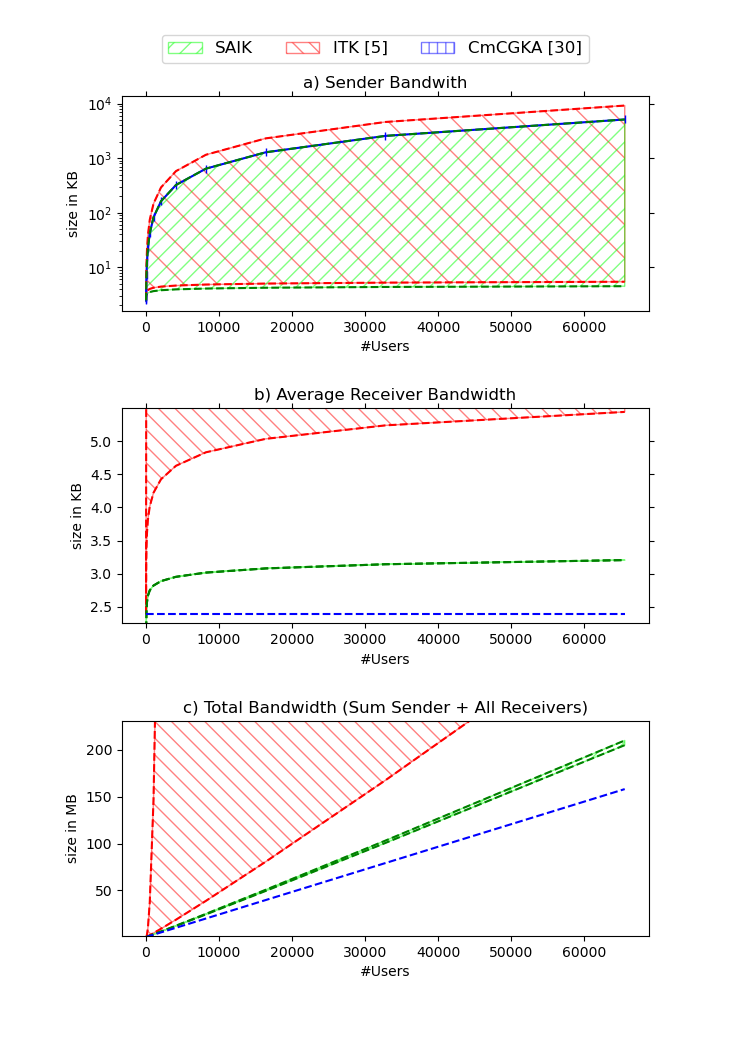
\includegraphics[width=\linewidth]{../plots/Final_Figures_Total}\end{minipage}\vspace*{-1cm}
	\caption{Bandwidth comparison of \saik, \protITK and \protCMPKE (instantiated with 256-bit
		security). Lower lines denote the tree-best-case execution history, while upper lines denote the
		tree-worst-case. All other possible cases are marked as the regions between the lines. Plot (a) shows the sender
        bandwidth on a \emph{log scale} and plot 
		(b) shows average individual receiver bandwidth on a \emph{linear scale}. Plot (c) shows the total bandwidth,
        i.e. the sum of sender bandwidth and $n$ times the receiver bandwidth. Note that in the first plot, the lines for tree-worst-case \saik and
		all-case \protCMPKE coincide.
		%Sender and receiver bandwidth for a group of size $N$ expressed as the (approximate) number of group elements.
	}
	\label{tab:plots}
  \end{minipage}
  \hfill
  \begin{minipage}[t]{.48\textwidth}
    \centering\vspace*{-9.5cm}
    \begin{minipage}[t]{\linewidth}
    	\begin{tabulary}{\linewidth}{|l|l|l|l|l|}
    		\hline
    		\multicolumn{2}{|c|}{}& \protITK & \saik & \protCMPKE \\
    		\hline
    		\multirow{2}{*}{Sender} 
    		& best case & $3\log(N)$ & $2\log(N)$ & $N$ \\\cline{2-5}
    		& worst case &$2N$ & $N$ & $N$ \\\hline
    		\multirow{2}{*}{\parbox{1.5cm}{(Maximum)\\receiver}} 
    		& best case & $3\log(N)$ & $\log(N)$&  $3$ \\\cline{2-5}
    		& worst case & $2N$ & $\log(N)$ & $3$ \\ \hline
            \multirow{2}{*}{Total}
            & best case & $3N\log(N)$ & $N\log(N)$ & $4N $ \\\cline{2-5}
            & worst case & $2N^2$ & $N\log(N)$ & $4N$ \\
    		\hline
    	\end{tabulary}
    \caption{
    	Sender, receiver and total bandwidth for a group of size $N$ expressed as the (approximate) number of group
        elements. Best/Worst case refers to the state of the tree, while we always consider the average receiver
        bandwidth over all receivers.
    }\label{fig:bandwidth2}
  \end{minipage}


  \begin{minipage}[t]{\linewidth}\centering
    \begin{tabulary}{\linewidth}{|l|r|}
      \hline
      & Bitsize \\
      \hline
      Group element & 512 \\
      \hline
      Hash & 512 \\
      \hline
      Signature & 1024 \\
      \hline
      Header & 17784 \\
      \hline
      \pkSize & 512 \\
      \hline
      \ctxSize & 1152 \\
      \hline
      $\mCtxSize(N)$ & $512 + N \cdot 640$ \\
      \hline
    \end{tabulary}
    \caption{Bitsizes used to generate \cref{tab:plots}. The header consists of the sender's id, the epoch id and some
      authenticated data required by the protocol. The individual ciphertexts consist of a group element and an AEAD
      encryption, while the \mPKE ciphertext all share the same group element. The header contains signatures, tags,
      epoch and sender identifier as well as a key package. The latter makes up the bulk of the header, as it contains
      credentials, more public keys and some application data. Our estimation is based on MLS.}
    \label{tab:bits}
  \end{minipage}
  \end{minipage}
\end{figure*}
\paragraph{Results.}
We estimated the bandwidth for all protocols using the formulas in \cref{tab:bandwidth1,fig:bandwidth2} with bit lengths
indicated in \cref{tab:bits}. This is further visualized in \cref{tab:plots} for growing group sizes $N$.
We highlight some interesting observations. % features of the plots. %For concreteness, we fix $N = 10K$ users.

In terms of the sender bandwidth, \saik is always at least as good as the other protocols. 
For example, in a group of 10K parties, \saik sender's require between $83\%$ and $55\%$ of the bandwidth of \protITK (due to the smaller mmPKE ciphertexts compared to PKE). \saik's tree-worst-case sender bandwidth is the same as \protCMPKE but its tree-best-case bandwidth can be as small as $0.52\%$ by using only $4$KB in stead of \protCMPKE's $783$KB. (Recall that, unlike in \protCMPKE, in \saik sender bandwidth varies depending on the history of preceding operations.)


In terms of the maximum receiver bandwidth, \protITK is much worse than \saik and \protCMPKE. For
example, \saik receivers (at most) need between $62\%$ (tree-best-case execution) to about $.2\%$ (tree-worst-case
execution) of \protITK's. On the other hand, \protCMPKE is the best for receivers.  \saik requires up
to $126\%$ of \protCMPKE's bandwidth, i.e. an increase from $\sim 2.4$KB to $\sim 3.02$KB for 10K parties.

Finally, the total bandwidth is by far the smallest for \protCMPKE and by far the largest for \protITK. For instance,
for 10K parties, \saik requires $\sim1.3$ times more total bandwidth, while \protITK requires anywhere from $\sim2$
times (tree-best-case) to $\sim50$ times (tree-worse-case) more.

In summary, the results show that \saik achieves the lowest bandwidth required from a single client
(i.e. $\bigO(\log(N))$ for \saik vs. $\bigO(N)$ for \protCMPKE), while \protCMPKE has the lowest total bandwidth
(i.e. $\bigO(N\log(N))$ for \saik vs. $\bigO(N)$ for \protCMPKE). (Hence, both protocols meet their design goals.) For instance, for 10K parties, \protCMPKE requires a client to upload $783$KB of data, while in scenarios close to the tree-best-case (which we believe to occur most of the time), the sender or receiver bandwidth of \saik is roughly $4$KB. On the other hand, the total bandwidth is roughly $25$MB for \protCMPKE and $30$MB for \saik.

\paragraph{Server computation.}
Lastly, we consider the server-side computation for \saik and \protCMPKE. In \protCMPKE, the server only picks the
$i$-th \mPKE ciphertext for the $i$-th user and forwards all common data. For \saik, we can consider two possibilities:
Either the server keeps track of the shape of the ratchet tree (which it can do based on the header data sent in all
packages) and computes the lowest common ancestor of sender and receiver in the tree, computes its resolution and then
forwards the corresponding ciphertext and public keys. This takes at most logarithmic time in the size of the
group (however, no expensive public-key operations are required). Alternatively, the user can compute its indices in the
tree and send them to the server, reducing the server computation to effectively the same as in \protCMPKE at the cost
of an additional round of communication.

%%% Local Variables:
%%% mode: latex
%%% TeX-master: "main"
%%% End:
